%This work is licensed under the Creative Commons License Attribution 4.0 International (CC-BY 4.0)
%https://creativecommons.org/licenses/by/4.0/legalcode
\documentclass[rgb]{standalone}
\usepackage{tkz-euclide}
\usepackage{amsmath}
\definecolor{myorange}{hsb}{0.0833, 1, 0.8}
\definecolor{mygreen}{hsb}{0.3333, 1, 0.8}
\definecolor{myblue}{hsb}{0.5833, 1, 0.8}
\definecolor{mymagenta}{hsb}{0.8333, 1, 0.8}
\begin{document}
	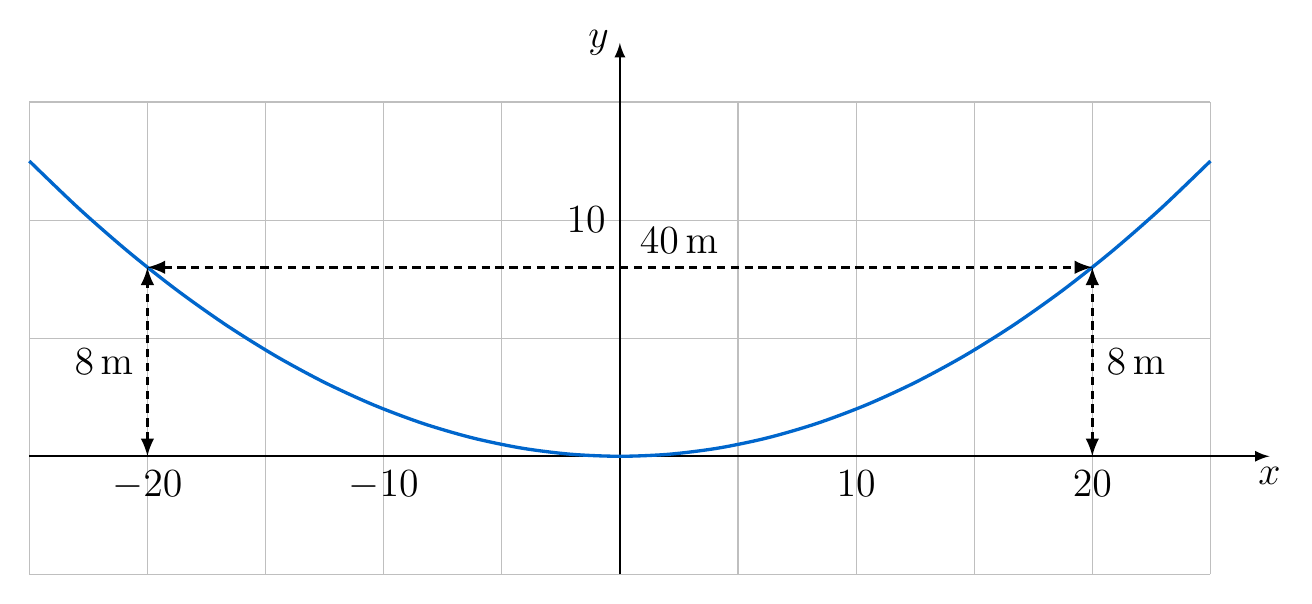
\begin{tikzpicture}[scale=1.5, font=\Large]
		% Coordinate system
		\tkzInit[xmin=-5,xmax=5,ymin=-1,ymax=3,xstep=1,ystep=1]
		\tkzGrid[color=lightgray]
		\tkzDrawX[thick,label=$x$]
		\tkzDrawY[thick,label=$y$]
		% Graph
		\draw[very thick,domain=-5:5, smooth, variable=\x, myblue] plot ({\x}, {1/10*\x*\x});
		\draw[very thick,densely dashed,latex-latex] (-4,0) -- (-4,1.6);
		\draw[very thick,densely dashed,latex-latex] (4,0) -- (4,1.6);
		\draw[very thick,densely dashed,latex-latex] (-4,1.6) -- (4,1.6);
		% Labels
		\node[below=0.5mm] at (-4,0){$-20$};
		\node[below=0.5mm] at (-2,0){$-10$};
		\node[below=0.5mm] at (2,0){$10$};
		\node[below=0.5mm] at (4,0){$20$};
		\node[left=0.5mm] at (0,2){$10$};
		\node[left=0.5mm] at (-4,0.8){$8\,\text{m}$};
		\node[right=0.5mm] at (4,0.8){$8\,\text{m}$};
		\node[above=0.5mm] at (0.5,1.6){$40\,\text{m}$};
	\end{tikzpicture}	
\end{document}